\section{link.h File Reference}
\label{link_8h}\index{link.h@{link.h}}
{\tt \#include \char`\"{}simulator.h\char`\"{}}\par
{\tt \#include $<$list$>$}\par
{\tt \#include $<$iostream$>$}\par
{\tt \#include $<$stdint.h$>$}\par


Include dependency graph for link.h:\nopagebreak
\begin{figure}[H]
\begin{center}
\leavevmode
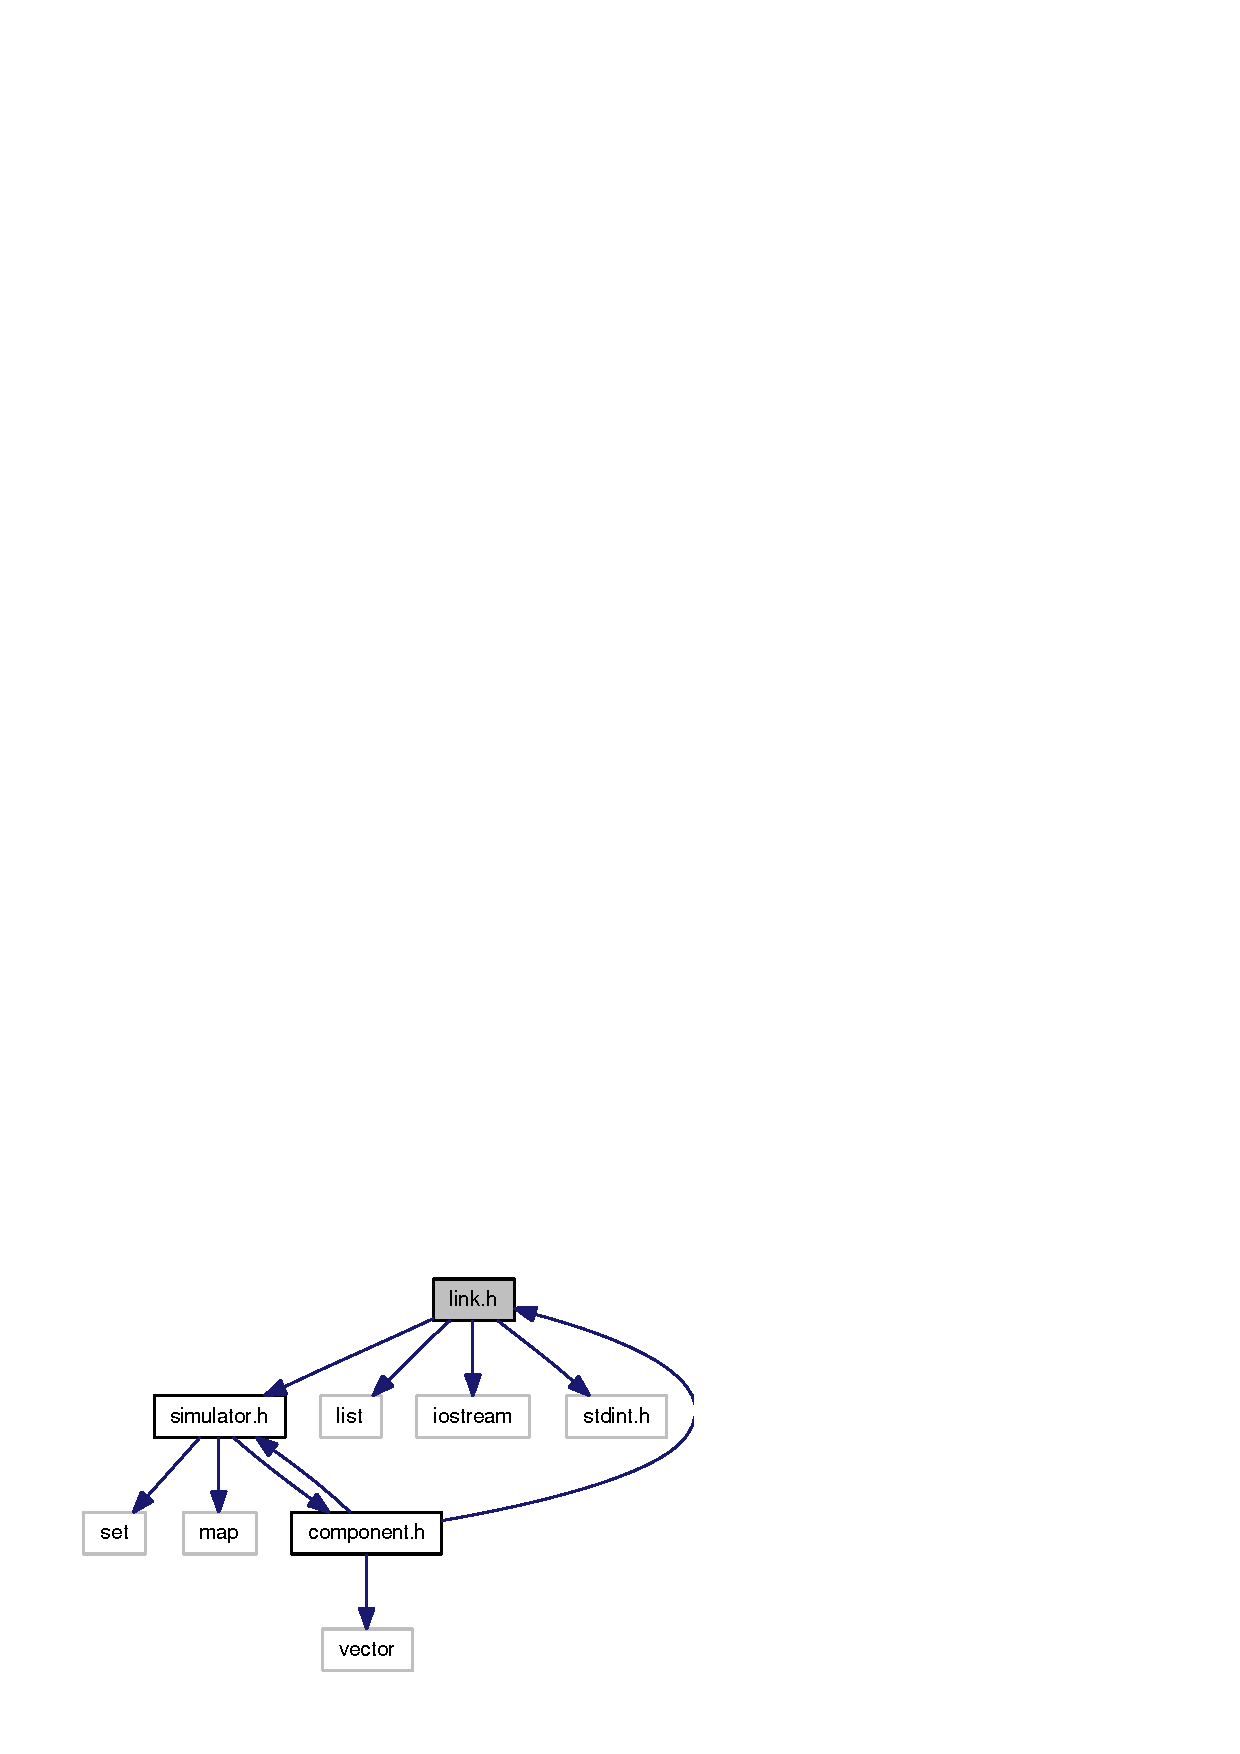
\includegraphics[width=166pt]{link_8h__incl}
\end{center}
\end{figure}


This graph shows which files directly or indirectly include this file:\nopagebreak
\begin{figure}[H]
\begin{center}
\leavevmode
\includegraphics[width=420pt]{link_8h__dep__incl}
\end{center}
\end{figure}
\subsection*{Classes}
\begin{CompactItemize}
\item 
class {\bf OutputBase}
\item 
class {\bf Output0$<$ OBJ $>$}
\item 
class {\bf Link}
\end{CompactItemize}
\subsection*{Functions}
\begin{CompactItemize}
\item 
{\footnotesize template$<$typename OBJ $>$ }\\void {\bf addOutput} ({\bf Link} $\ast$l, int outComponent, double latency, void(OBJ::$\ast$f)(uint64\_\-t, int), OBJ $\ast$obj0)
\end{CompactItemize}


\subsection{Function Documentation}
\index{link.h@{link.h}!addOutput@{addOutput}}
\index{addOutput@{addOutput}!link.h@{link.h}}
\subsubsection[{addOutput}]{\setlength{\rightskip}{0pt plus 5cm}template$<$typename OBJ $>$ void addOutput ({\bf Link} $\ast$ {\em l}, \/  int {\em outComponent}, \/  double {\em latency}, \/  void(OBJ::$\ast$)(uint64\_\-t, int) {\em f}, \/  OBJ $\ast$ {\em obj0})\hspace{0.3cm}{\tt  [inline]}}\label{link_8h_5d79dd8efc21ef444d3a96cdd9f522ab}




Definition at line 49 of file link.h.

References Link::outputs.